\documentclass[10pt,twocolumn,letterpaper]{article}

\usepackage{cvpr}
\usepackage{times}
\usepackage{epsfig}
\usepackage{graphicx}
\usepackage{amsmath}
\usepackage{amssymb}

% Include other packages here, before hyperref.

% If you comment hyperref and then uncomment it, you should delete
% egpaper.aux before re-running latex.  (Or just hit 'q' on the first latex
% run, let it finish, and you should be clear).
\usepackage[breaklinks=true,bookmarks=false]{hyperref}

\cvprfinalcopy % *** Uncomment this line for the final submission

\def\cvprPaperID{****} % *** Enter the CVPR Paper ID here
\def\httilde{\mbox{\tt\raisebox{-.5ex}{\symbol{126}}}}

% Pages are numbered in submission mode, and unnumbered in camera-ready
\ifcvprfinal\pagestyle{empty}\fi
% \setcounter{page}{4321}
\begin{document}


%%%%%%%%% TITLE
\title{draw2pix: Generative Adversarial Networks for Art School Rejects}

\author{Cedrick Argueta\\
Stanford University\\
450 Serra Mall, Stanford, CA 94305\\
{\tt\small cedrick@cs.stanford.edu}
% For a paper whose authors are all at the same institution,
% omit the following lines up until the closing ``}''.
% Additional authors and addresses can be added with ``\and'',
% just like the second author.
% To save space, use either the email address or home page, not both
\and
Kevin Wang\\
Stanford University\\
450 Serra Mall, Stanford, CA 94305\\
{\tt\small kwang98@stanford.edu}
}

\maketitle
%\thispagestyle{empty}

%%%%%%%%% BODY TEXT
\section{Introduction}
We are investigating unpaired image-to-image translation with generative adversarial networks.
This work was demonstrated in \cite{cycleGAN}.
Work done in the same lab \cite{pix2pix} demonstrates how we can use paired images in training to create an image-to-image mapping from one domain to another.
The specific image-to-image task that we're aiming to implement is \href{https://affinelayer.com/pixsrv/}{this}, which demonstrates a couple examples of sketch-to-photo translations trained using the pix2pix model.
We aim to do something similar, using CycleGAN to instead train on unpaired images.
The relaxation that unpaired training gives us allows for easier creation of datasets and combinations of domains -- we can simply swap a whole domain and retrain rather than find image-to-image pairs for that specific translation task.
Our project differs from \cite{bicyclegan} in that we aren't doing multi-modal image translation, just from one domain to another. 
We are essentially implementing the demo from \cite{pix2pix} with an unpaired dataset and architecture matching that of \cite{cycleGAN}

\section{Related Work}
% TODO: gan, cogan citation
The original Generative Adversarial Network (GAN) proposed by Goodfellow et al. \cite{gan}  proposes a network that learns an approximation of a distribution of data $p_{X}$.
It does so by training two networks - a generator network and a discriminator network.
These networks are trained adversarially, i.e. the discriminator's objective is to discern between real images and the generator's images, and the generator's objective is to generate images that fool the discriminator.

Generative networks are not limited to simple distributions.
Work done by Liu et al. \cite{cogan} demonstrated the ability of generative networks to learn a joint distribution between variables, through the use of multiple generator and discriminator networks.
This can be used to generate pairs $x_1 \sim p_{X_1}, x_2 \sim p_{X_2}$ of images that belong to the joint distribution just by using the marginal distributions.

Zhu et al. \cite{cycleGAN} goes a step further by enforcing cycle consistency between pairs created, i.e. by ensuring that generated images can be run through another generator to create the paired image.
CycleGAN effectively learns a mapping function $G : X \rightarrow Y$ for images in domains $X$ and $Y$.

CycleGAN in particular does unsupervised image-to-image translation in that no labels are given to pair images from domain $X$ and domain $Y$ together.
When these labels are given, supervised methods like those described by Isola et al. \cite{pix2pix} are possible through the use of conditional GANs.

\section{Problem Statement}
The problem we are addressing is image-to-image translation from an input domain $X$ of hand-drawn tree sketches to the output domain $Y$ of realistic photographs of trees. Specifically, we are working with unpaired training data, meaning there is no mapping between sketches $x_i\in X$ and target photos $y_j \in Y$. Often, finding paired data for the image-to-image translation task is difficult. Moreover, using unpaired image data allows for independent collection of input and output training sets. This motivates the problem that we are attempting to solve.


\section{Technical Approach}
We aim to use CycleGAN \cite{cycleGAN} for unpaired image-to-image translation.
More precisely, we will train networks to learn functions $G : X \rightarrow Y$ and $F: Y \rightarrow X$.
This will allow us to take an image $x_1 \in X$ and generate its pair $y_1 \in Y$, and vice versa.
We let the true distributions of the domains be $p_X$ and $p_Y$.
Just as in \cite{gan}, we will use discriminators $D_X$ and $D_Y$ as adversarial networks to the generators, which we will train to distinguish between elements in $X$ and $p_X$ and $Y$ and $p_Y$, respectively.
CycleGAN uses two losses per generator function.
The first loss is adversarial, where the loss function for $G$ and its discriminator $D_Y$ is:
\begin{equation}
\begin{split}
\displaystyle \mathcal{L}_{GAN}(G, D_Y, X, Y) = 
\mathbb{E}_{y \sim p_Y}[\log{D_Y(y)}]
\\ + \mathbb{E}_{x \sim p_X}[\log{(1 - D_Y(G(x)))}]
\end{split}
\end{equation}
and the objective is $\displaystyle \min_{G} \max_{D_Y} \mathcal{L}_{GAN}$.
We can apply this without loss of generality to $F$ and its discriminator $D_X$.
Because it is possible for a network to map an input image $x$ to multiple images in $Y$, we use a cycle consistency loss to guarantee that there is a unique mapping.
Specifically, we wish to enforce that for images $x$ and $y$ $F(G(x)) \approx x$ (forward cycle consistency) and $G(F(y)) \approx y$ (backward cycle consistency).
The loss used is:
\begin{equation}
\begin{split}
\displaystyle \mathcal{L}_{cyc} = 
\mathbb{E}_{x \sim p_X}[\Vert{F(G(x)) - x}\Vert_1]
\\ + \mathbb{E}_{y \sim p_Y}[\Vert{G(F(y)) - y}\Vert_1]
\end{split}
\end{equation}

Then the full loss function is:
\begin{equation}
\begin{split}
\displaystyle \mathcal{L}(G, F, D_X, D_Y) = 
\mathcal{L}_{GAN}(G, D_Y, X, Y)
\\+ \mathcal{L}_{GAN}(F, D_X, Y, X)
\\+ \lambda\mathcal{L}_{cyc}(G, F)
\end{split}
\end{equation}
where $\lambda$ is a parameter that determines the importance of cyclic consistency loss vs. adversarial loss.
Minimizing this loss through
\begin{equation}
\displaystyle G^*, F^* = \arg\min_{G, F}\max_{D_X, D_Y} \mathcal{L}(G, F, D_X, D_Y)
\end{equation}
yields $G^*$ and $F^*$, our optimal mapping functions.
\section{Dataset}
We will be using a subset of the Sketchy dataset, as described in \cite{sangkloy2016sketchy}. The dataset consists of a crowd-sourced collection of sketch-photo pairs. The total collection consists of 75,471 sketches of 12,500 photos (125 object categories). We will be working specifically with the 'tree' subset, which consists of 100 photos and 534 sketches. Although there is a naturally defined pairing between photos and sketches, we will be ignoring this mapping in our implementation of unpaired translation. Currently, we are preprocessing both domains in our baseline by zero-centering and scaling pixel values to the [-1, 1] range. We are planning on normalizing data for both domains in our implementation of CycleGAN as well.

\section{Baseline Results}
We use CoGAN \cite{cogan} as a baseline since it is a simpler model that can also learn joint distributions.
Our method with CoGAN is to learn the joint distribution of images from $p_X$ and $p_Y$, where $p_X$ and $p_Y$ are the marginal distributions of tree sketches and tree photos, respectively.
CoGAN allows us to learn $G_X$ and $G_Y$, generative models that allow us to synthesize new images in the distributions $X$ and $Y$.
Since these networks are coupled, i.e. they share parameters in the decoding section of the generator and in the encoding section of the discriminator, we can use both to learn a mapping between $X$ and $Y$.
For a given input $x$, we must find a noise vector $z^*$ such that $G_X(z^*) \approx x$.
The corresponding image $y$ is then just $G_Y(z^*)$.

% \begin{figure}
%   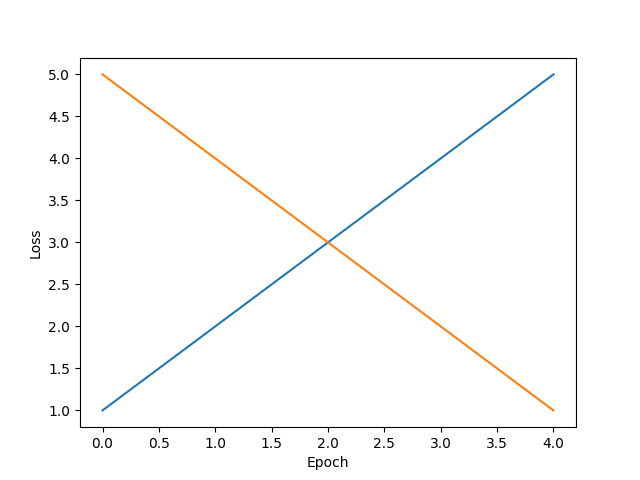
\includegraphics[width=\linewidth]{loss.png}
%   \caption{Discriminator and generator loss curves for our best model.}
%   \label{cogan_loss}
% \end{figure}

At the moment, our baseline results are almost completely unsuccessful.
While Zhu et al. \cite{cycleGAN} note that CoGAN was relatively unsuccessful at producing realistic mappings, our generators fail to capture any semblance of the target domain.
We suspect that this is due to the lack of a large dataset, leading us to believe that we need data augmentation (rotations, jitter for the real photos, etc.).
We may also augment our dataset with edge maps of other images of trees, giving us more variance and a larger dataset that would prove invaluable.
We also underestimated the difficulty of training generative networks, where we found ourselves struggling with hyperparameters and tricks to get the loss values to converge.
Oftentimes we find that either the generator or the discriminator will begin to dominate the other network early on in training, and finding the perfect balance of learning rates, ratio of number of updates, and architecture is extremely difficult.
We realize that we will need much longer training times and a better strategy for encouraging the loss functions to converge.
% The loss functions for the generators and discriminators in our CoGAN approach can be seen in \ref{cogan_loss}.

The CoGAN model fails to produce images that can be recognized as realistic trees, with most images qualitatively looking like random noise.
Some images of produced outputs at different epochs can be seen in \ref{cogan_pics}.

\begin{figure}
  \includegraphics[width=\linewidth]{../../first_images/100.png}
  \includegraphics[width=\linewidth]{../../first_images/99000.png}
  \caption{Generated images after 100 epochs and 99000 epochs.}
  \label{cogan_pics}
\end{figure}

Despite these shortcomings, we check out generated images using the Fr\'echet Inception Distance.
The Fr\'echet Inception Distance compares activation distributions of generated samples vs. real samples on the InceptionV3 network.
For this metric, lower is better.
Our generated images for sketches of trees received an FID score of 526.59 with our best model, while generated images for real trees received an FID score of 538.97.
We hope to dramatically reduce these scores in the next few days, as we need a decent and functional baseline to even compare against CycleGAN on the same task.
For perspective, other implementations of GANs trained on other datasets can achieve FID scores well below 100, sometimes even below 20.

Next, we will improve on our CoGAN implementation so that we will have a suitable baseline to compare CycleGAN to.
Prior to this, however, we will need to address issues with our dataset, namely the lack of a large enough dataset to get a decent generative model.
We will also implement CycleGAN, another network that can perform unpaired image-to-image translation, and compare the results to CoGAN and hopefully be able to use a hand-drawn sketch of a tree to create a photorealistic tree.
{\small
\bibliographystyle{ieee}
\bibliography{ref}
}

\end{document}
